\documentclass{beamer}
\usetheme{Madrid}
\usepackage{tikz}
\usetikzlibrary{shapes,arrows,positioning,calc,backgrounds,matrix,fit}

\begin{document}

\begin{frame}[fragile]
\begin{center}
  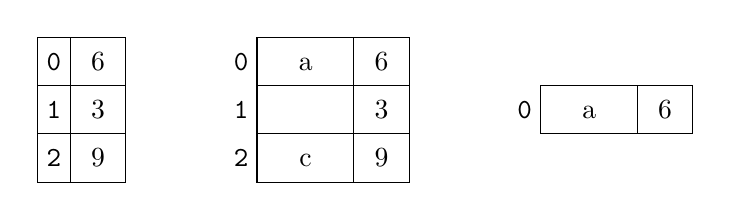
\begin{tikzpicture}[
    cell/.style={rectangle,draw=black},
    space/.style={minimum height=1.5em,
                  matrix of nodes,
                  row sep=-\pgflinewidth,
                  column sep=-\pgflinewidth,
                  column 1/.style={font=\ttfamily}},
    text depth=0.5ex,
    text height=2ex,
    nodes in empty cells]

    \matrix (first) [
      space,
      column 1/.style={nodes=cell,font=\ttfamily},
      column 2/.style={nodes={cell,minimum width=2em}}]
    {
      0   & 6 \\
      1   & 3 \\
      2   & 9 \\
    };

    \matrix (second) [
      right=of first,
      space,
      column 2/.style={minimum width=3em,nodes={cell,minimum width=3.5em}},
      column 3/.style={nodes={cell,minimum width=2em}}]
    {
      0   &a  & 6 \\
      1   &   & 3 \\
      2   &c  & 9 \\
    };

    \matrix [
      right=of second,
      space,
      column 2/.style={minimum width=3em,nodes={cell,minimum width=3.5em}},
      column 3/.style={nodes={cell,minimum width=2em}}]
    {
      0   &a  & 6 \\
%      1   &b  & 3 \\
%      2   &c  & 9 \\
    };
  \end{tikzpicture}
\end{center}
\end{frame}

\end{document}
